% =============================================================================
% شکل‌های کیفی — خروجی tools/make_qualitative_figure.py (پروتکل پیش‌ثبت‌شده)
%
% فایل‌های لازم:
%   thesis/figures/qualitative_depth_maps.pdf
%   thesis/figures/curves/scale_ratio_hist.csv
%
% محل درج: انتهای بخش ۴--۶، با دستور:
%   % =============================================================================
% شکل‌های کیفی — خروجی tools/make_qualitative_figure.py (پروتکل پیش‌ثبت‌شده)
%
% فایل‌های لازم:
%   thesis/figures/qualitative_depth_maps.pdf
%   thesis/figures/curves/scale_ratio_hist.csv
%
% محل درج: انتهای بخش ۴--۶، با دستور:
%   % =============================================================================
% شکل‌های کیفی — خروجی tools/make_qualitative_figure.py (پروتکل پیش‌ثبت‌شده)
%
% فایل‌های لازم:
%   thesis/figures/qualitative_depth_maps.pdf
%   thesis/figures/curves/scale_ratio_hist.csv
%
% محل درج: انتهای بخش ۴--۶، با دستور:
%   % =============================================================================
% شکل‌های کیفی — خروجی tools/make_qualitative_figure.py (پروتکل پیش‌ثبت‌شده)
%
% فایل‌های لازم:
%   thesis/figures/qualitative_depth_maps.pdf
%   thesis/figures/curves/scale_ratio_hist.csv
%
% محل درج: انتهای بخش ۴--۶، با دستور:
%   \input{./figures/pending/qualitative_figures}
%
% سرستون‌های فارسی در همین‌جا حروف‌چینی می‌شوند (نه داخل تصویر)، تا با
% تایپوگرافی بقیهٔ پایان‌نامه یکسان باشند. کسرهای افقی زیر، دقیقاً همان
% COLUMN_CENTRES در tools/make_qualitative_figure.py هستند؛ اگر هندسهٔ آن
% اسکریپت تغییر کند، این چهار عدد نیز باید به‌روزرسانی شوند.
% =============================================================================

\begin{figure}[htbp]
    \centering
    \begin{tikzpicture}
        \node[anchor=south west, inner sep=0pt] (maps)
            {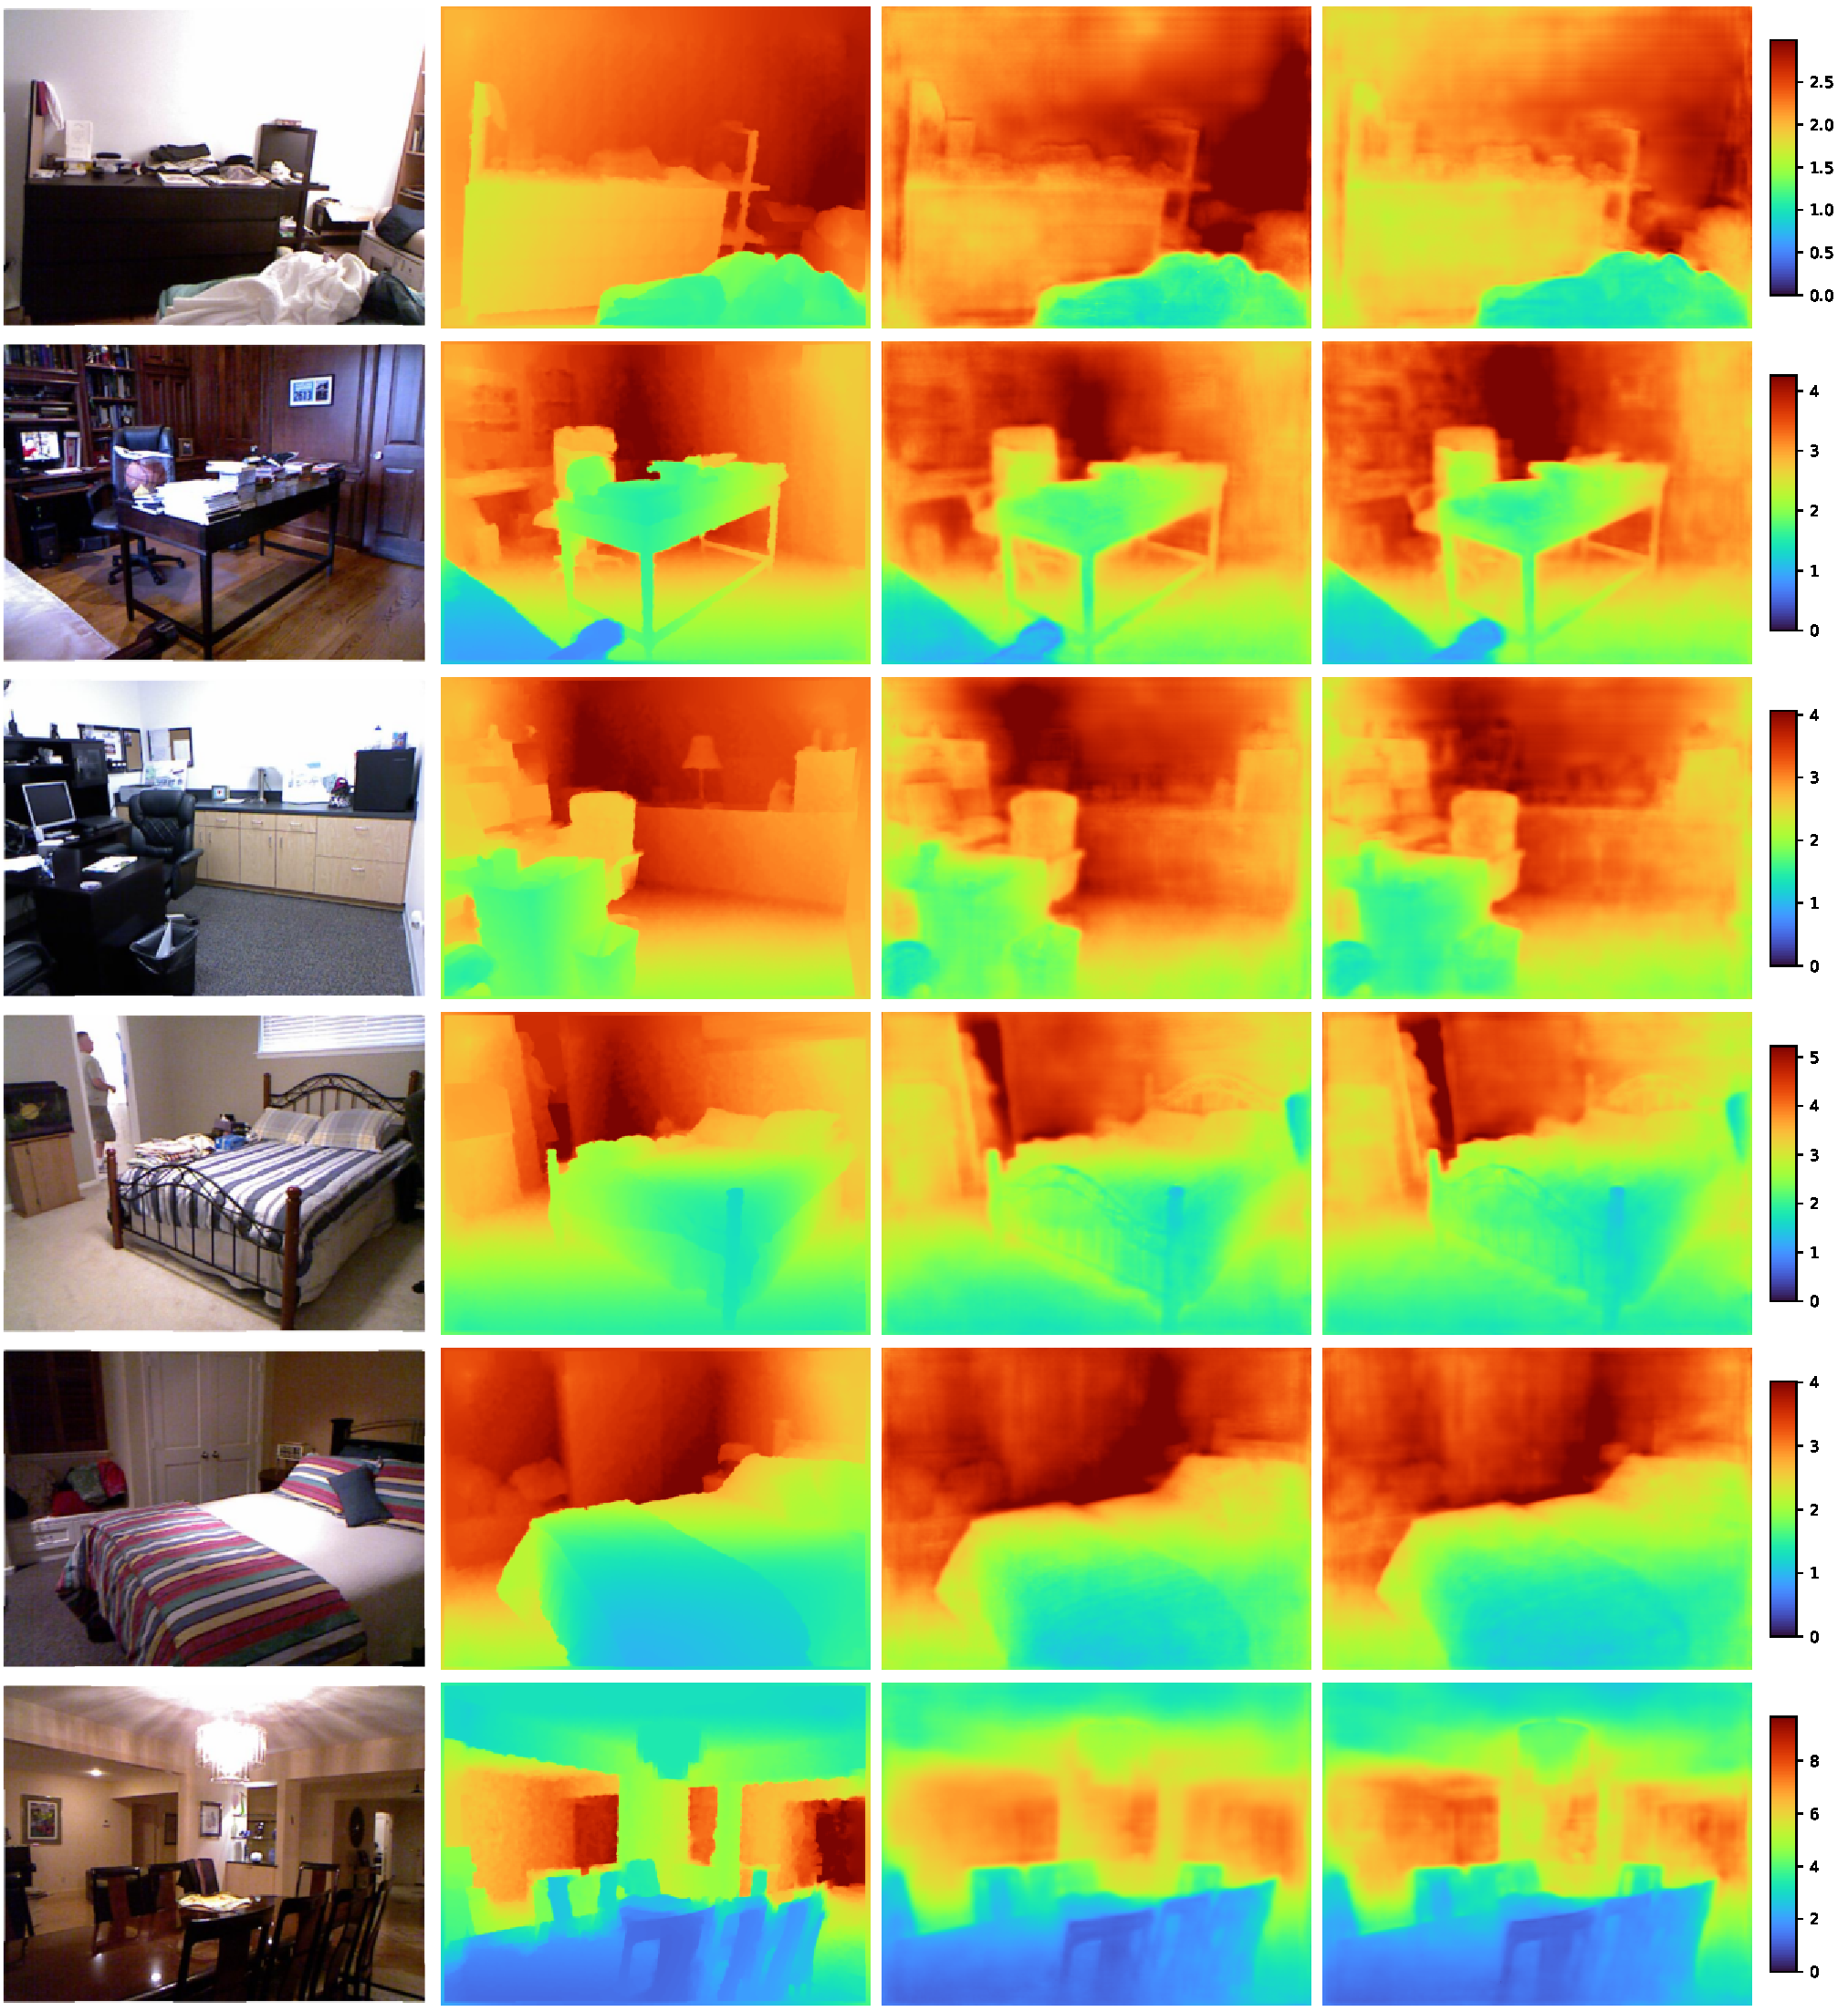
\includegraphics[width=\textwidth]{./figures/qualitative_depth_maps.pdf}};
        \node[thnote, anchor=south, font=\scriptsize\bfseries]
            at ([xshift=0.11625\textwidth]maps.north west) {تصویر ورودی};
        \node[thnote, anchor=south, font=\scriptsize\bfseries]
            at ([xshift=0.35475\textwidth]maps.north west) {عمق مرجع};
        \node[thnote, anchor=south, font=\scriptsize\bfseries, text=thControl]
            at ([xshift=0.59325\textwidth]maps.north west) {\tablecontrolmodel{} (فاقد \lr{K})};
        \node[thnote, anchor=south, font=\scriptsize\bfseries, text=thProposed]
            at ([xshift=0.83175\textwidth]maps.north west) {\tableproposedmodel{} (دارای \lr{K})};
    \end{tikzpicture}
    \caption[مقایسهٔ کیفی روی نمونهٔ پیش‌ثبت‌شده]{مقایسهٔ کیفی خروجی
    \proposedmodel{} و \controlmodel{} روی نمونه‌ای که \emph{پیش از هرگونه
    استنتاج} قفل شده است. شش تصویر تنها از روی بذر تصادفی \fadecimal{۲۰۲۶۰۸۲۱}
    از میان ۶۵۴ تصویر مجموعهٔ آزمون انتخاب شدند و چکیدهٔ \lr{SHA-256} فهرست
    شناسه‌ها (\lr{8086cb124e40}) پیش از بارگذاری هر مدل ثبت شد؛ بنابراین
    گزینش پس از مشاهدهٔ نتایج ممکن نبوده و شکل قابل ممیزی است. ستون‌ها از
    چپ به راست: تصویر ورودی، عمق مرجع، خروجی \controlmodel{} و خروجی
    \proposedmodel{}. در هر ردیف، نگاشت رنگ و بازهٔ عمق برای مرجع و هر دو
    مدل \emph{یکسان} است (نوار رنگ سمت راست همان ردیف، برحسب متر)، تا هیچ
    برتری بصری از نرمال‌سازی جداگانهٔ هر تصویر ناشی نشود. تفاوت دو مدل عمدتاً
    در \emph{مقیاس مطلق} صحنه است، نه در جزئیات ساختاری --- که با سازوکار
    پیش‌بینی‌شده در بخش~\ref{subsec:focal_jitter} هم‌خوان است.}
    \label{fig:qualitative_locked}
\end{figure}

\begin{figure}[htbp]
    \centering
    \begin{tikzpicture}
    \begin{axis}[
        thesisplot,
        width=0.86\textwidth, height=6.6cm,
        xlabel={نسبت مقیاس هر تصویر: میانهٔ پیش‌بینی تقسیم بر میانهٔ مرجع},
        ylabel={تعداد تصاویر},
        xmin=0.70, xmax=1.60, ymin=0, ymax=105,
        xtick={0.7,0.8,0.9,1.0,1.1,1.2,1.3,1.4,1.5,1.6},
        legend style={at={(0.97,0.97)}, anchor=north east},
        legend cell align=left,
    ]
    \addplot[ybar, bar width=0.0235, bar shift=0pt, draw=thProposed,
             fill=thProposed, fill opacity=0.55, draw opacity=0.9]
        table[x=center, y=proposed, col sep=space] {figures/curves/scale_ratio_hist.csv};
    \addlegendentry{\tableproposedmodel{}؛ میانه $1.015$}
    \addplot[ybar, bar width=0.0235, bar shift=0pt, draw=thControl,
             fill=thControl, fill opacity=0.45, draw opacity=0.9]
        table[x=center, y=control, col sep=space] {figures/curves/scale_ratio_hist.csv};
    \addlegendentry{\tablecontrolmodel{}؛ میانه $1.041$}
    % خط ایده‌آل با forget plot رسم می‌شود تا وارد فهرست راهنما نشود؛ برچسب آن
    % به‌صورت یک گره در کنار خط می‌آید.
    \addplot[draw=thIdeal, thick, dashed, forget plot]
        coordinates {(1.0,0) (1.0,105)};
    \node[thnote, anchor=west, text=thIdeal] at (axis cs:1.02,99) {ایده‌آل $1.000$};
    \end{axis}
    \end{tikzpicture}
    \caption[توزیع نسبت مقیاس هر تصویر]{توزیع نسبت مقیاس هر تصویر روی
    \emph{تمام} ۶۵۴ تصویر مجموعهٔ آزمون --- همان نمونه‌ای که آزمون‌های زوجی
    بخش~\ref{subsec:focal_jitter} روی آن انجام شده است. مقدار ایده‌آل ۱ است.
    این نمودار سازوکار عددی برتری گزارش‌شده در
    جدول~\ref{tab:nyu_metric_focal} را آشکار می‌کند: توزیع \proposedmodel{}
    هم نزدیک‌تر به مقدار ایده‌آل است (میانه \fadecimal{۱٫۰۱۵} در برابر
    \fadecimal{۱٫۰۴۱}) و هم فشرده‌تر (انحراف معیار \fadecimal{۰٫۰۷۸} در برابر
    \fadecimal{۰٫۰۹۴}؛ دامنهٔ میان‌چارکی \fadecimal{۰٫۰۹۸} در برابر
    \fadecimal{۰٫۱۱۴}). به بیان دیگر، \controlmodel{} --- که ناچار است به
    میانگین توزیع $\alpha$ رگرسیون کند --- هم اریب است و هم پراکنده‌تر، دقیقاً
    همان‌گونه که تحلیل بدساختی مسئله پیش‌بینی می‌کرد. در سطح تک‌تصویر نیز،
    \proposedmodel{} در ۳۹۹ تصویر از ۶۵۴ تصویر (۶۱ درصد) به مقیاس صحیح
    نزدیک‌تر است.}
    \label{fig:scale_ratio_distribution}
\end{figure}

%
% سرستون‌های فارسی در همین‌جا حروف‌چینی می‌شوند (نه داخل تصویر)، تا با
% تایپوگرافی بقیهٔ پایان‌نامه یکسان باشند. کسرهای افقی زیر، دقیقاً همان
% COLUMN_CENTRES در tools/make_qualitative_figure.py هستند؛ اگر هندسهٔ آن
% اسکریپت تغییر کند، این چهار عدد نیز باید به‌روزرسانی شوند.
% =============================================================================

\begin{figure}[htbp]
    \centering
    \begin{tikzpicture}
        \node[anchor=south west, inner sep=0pt] (maps)
            {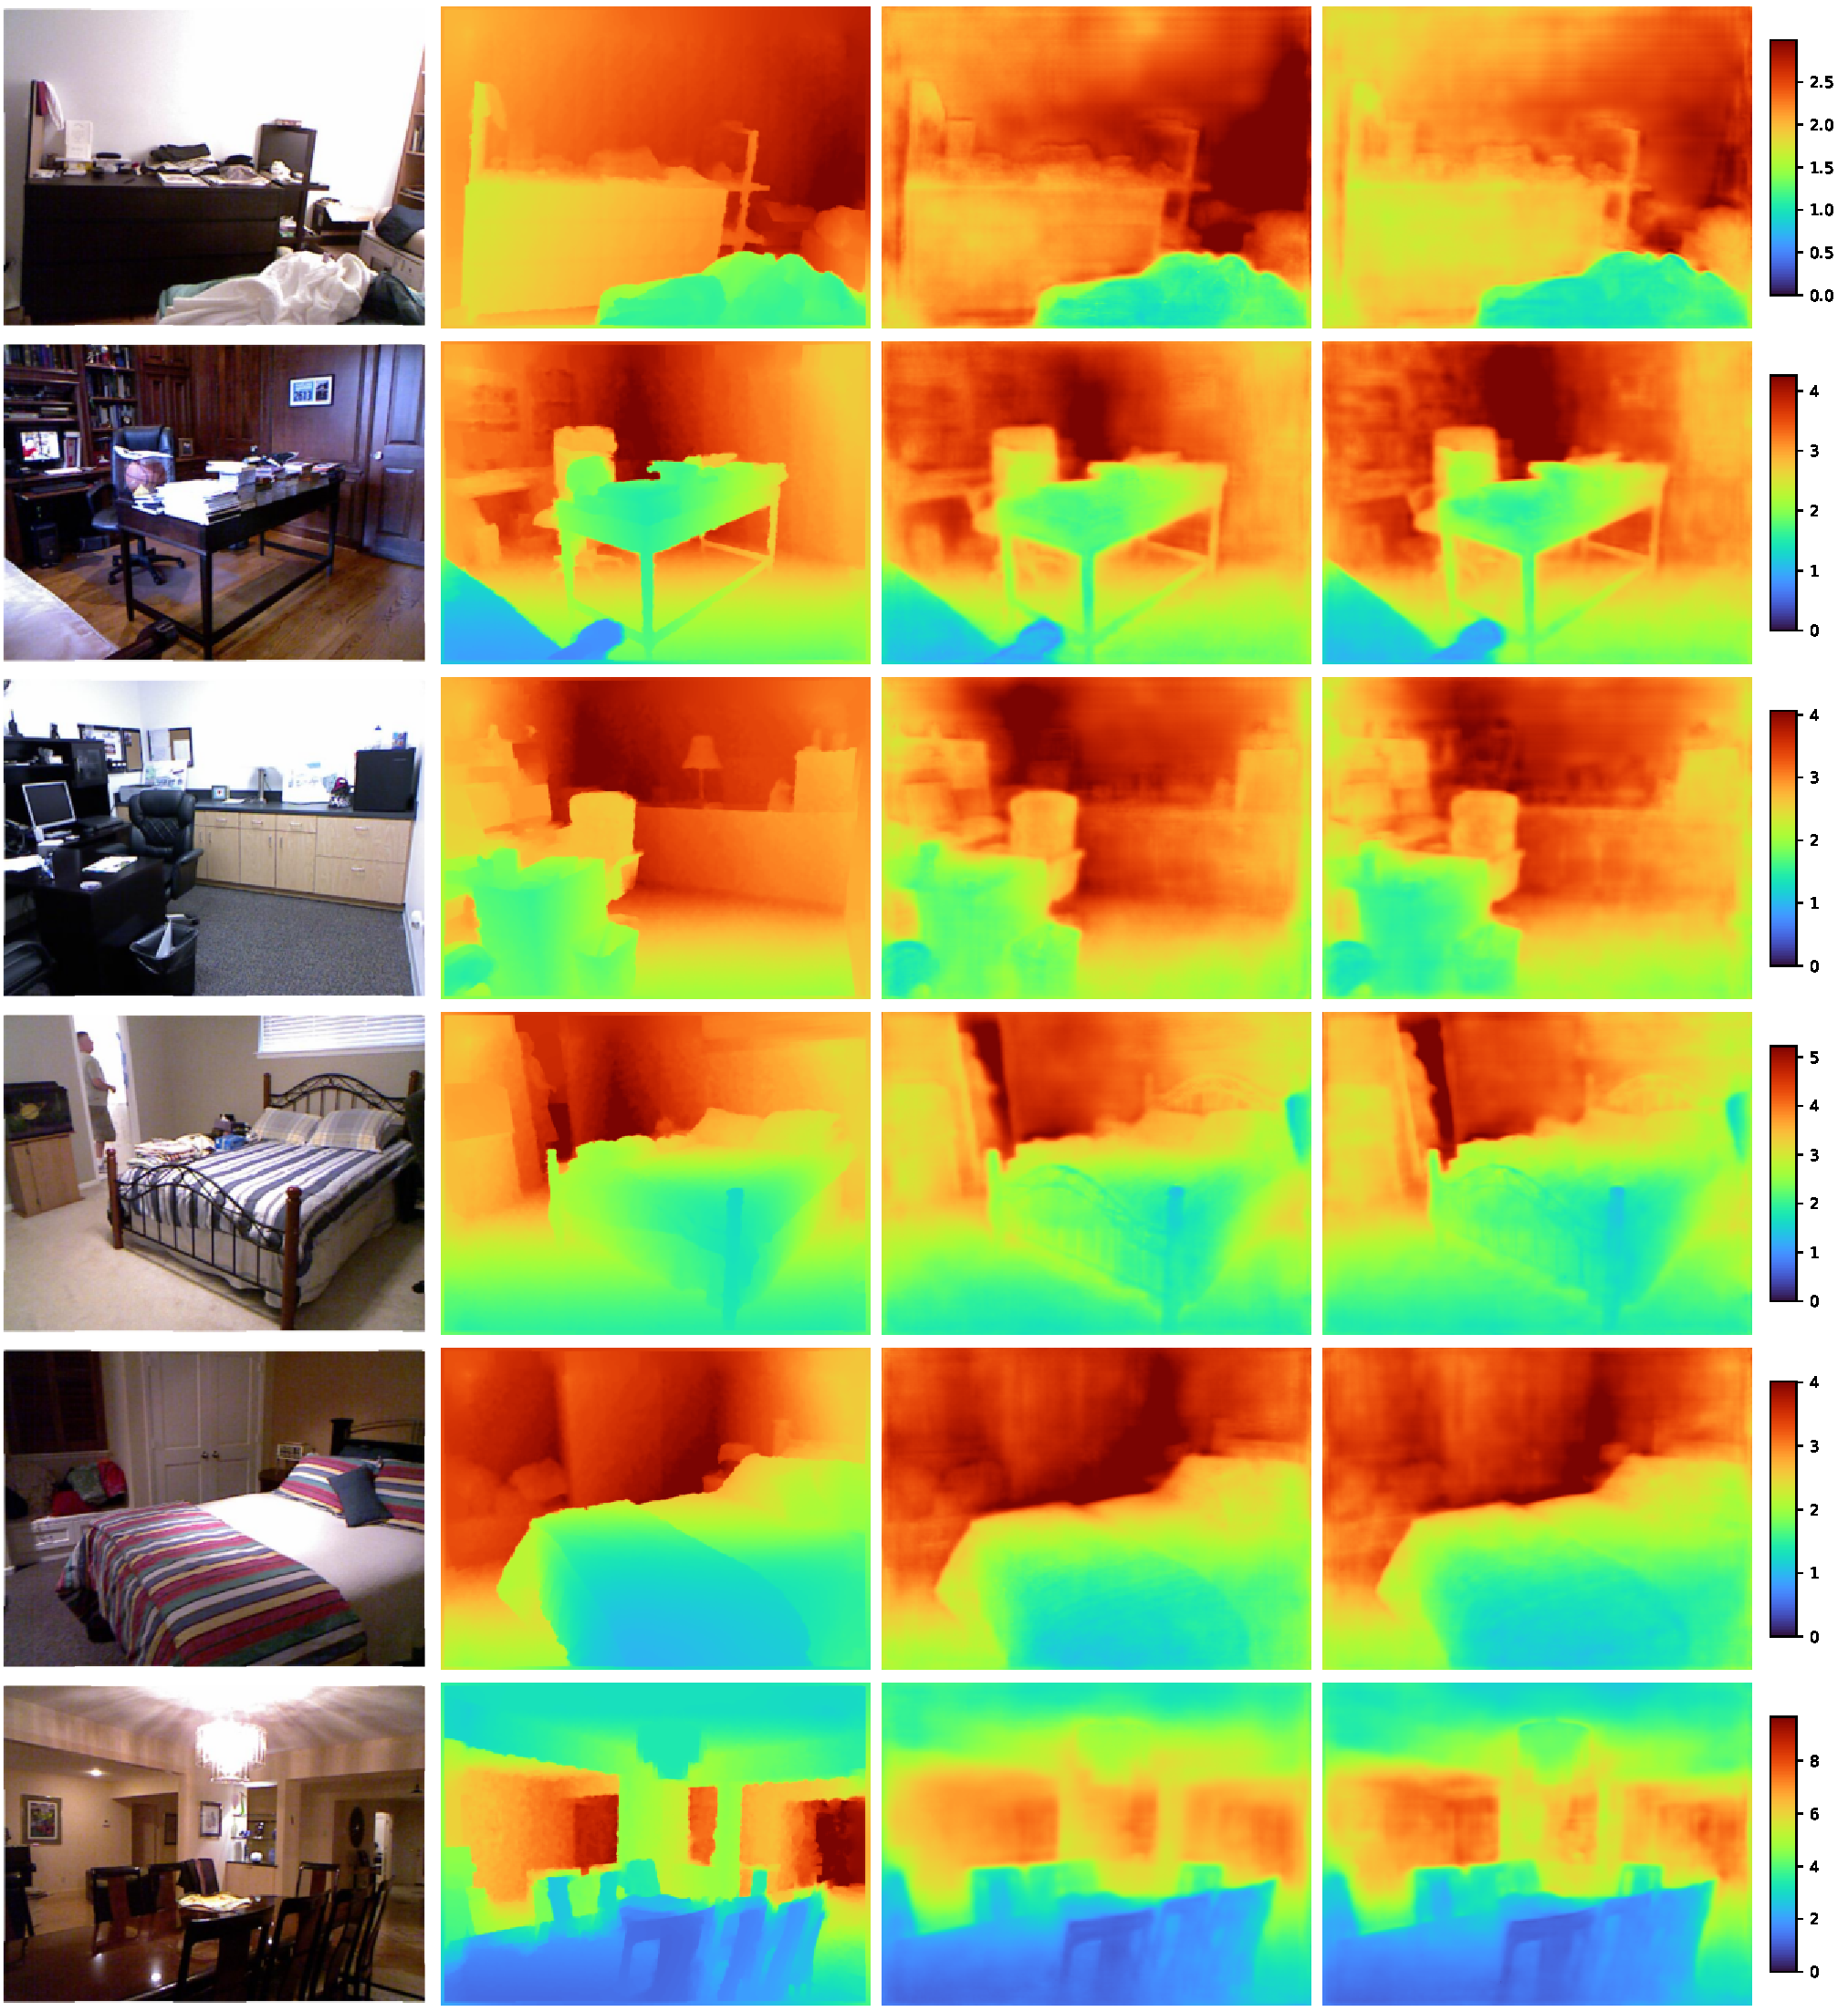
\includegraphics[width=\textwidth]{./figures/qualitative_depth_maps.pdf}};
        \node[thnote, anchor=south, font=\scriptsize\bfseries]
            at ([xshift=0.11625\textwidth]maps.north west) {تصویر ورودی};
        \node[thnote, anchor=south, font=\scriptsize\bfseries]
            at ([xshift=0.35475\textwidth]maps.north west) {عمق مرجع};
        \node[thnote, anchor=south, font=\scriptsize\bfseries, text=thControl]
            at ([xshift=0.59325\textwidth]maps.north west) {\tablecontrolmodel{} (فاقد \lr{K})};
        \node[thnote, anchor=south, font=\scriptsize\bfseries, text=thProposed]
            at ([xshift=0.83175\textwidth]maps.north west) {\tableproposedmodel{} (دارای \lr{K})};
    \end{tikzpicture}
    \caption[مقایسهٔ کیفی روی نمونهٔ پیش‌ثبت‌شده]{مقایسهٔ کیفی خروجی
    \proposedmodel{} و \controlmodel{} روی نمونه‌ای که \emph{پیش از هرگونه
    استنتاج} قفل شده است. شش تصویر تنها از روی بذر تصادفی \fadecimal{۲۰۲۶۰۸۲۱}
    از میان ۶۵۴ تصویر مجموعهٔ آزمون انتخاب شدند و چکیدهٔ \lr{SHA-256} فهرست
    شناسه‌ها (\lr{8086cb124e40}) پیش از بارگذاری هر مدل ثبت شد؛ بنابراین
    گزینش پس از مشاهدهٔ نتایج ممکن نبوده و شکل قابل ممیزی است. ستون‌ها از
    چپ به راست: تصویر ورودی، عمق مرجع، خروجی \controlmodel{} و خروجی
    \proposedmodel{}. در هر ردیف، نگاشت رنگ و بازهٔ عمق برای مرجع و هر دو
    مدل \emph{یکسان} است (نوار رنگ سمت راست همان ردیف، برحسب متر)، تا هیچ
    برتری بصری از نرمال‌سازی جداگانهٔ هر تصویر ناشی نشود. تفاوت دو مدل عمدتاً
    در \emph{مقیاس مطلق} صحنه است، نه در جزئیات ساختاری --- که با سازوکار
    پیش‌بینی‌شده در بخش~\ref{subsec:focal_jitter} هم‌خوان است.}
    \label{fig:qualitative_locked}
\end{figure}

\begin{figure}[htbp]
    \centering
    \begin{tikzpicture}
    \begin{axis}[
        thesisplot,
        width=0.86\textwidth, height=6.6cm,
        xlabel={نسبت مقیاس هر تصویر: میانهٔ پیش‌بینی تقسیم بر میانهٔ مرجع},
        ylabel={تعداد تصاویر},
        xmin=0.70, xmax=1.60, ymin=0, ymax=105,
        xtick={0.7,0.8,0.9,1.0,1.1,1.2,1.3,1.4,1.5,1.6},
        legend style={at={(0.97,0.97)}, anchor=north east},
        legend cell align=left,
    ]
    \addplot[ybar, bar width=0.0235, bar shift=0pt, draw=thProposed,
             fill=thProposed, fill opacity=0.55, draw opacity=0.9]
        table[x=center, y=proposed, col sep=space] {figures/curves/scale_ratio_hist.csv};
    \addlegendentry{\tableproposedmodel{}؛ میانه $1.015$}
    \addplot[ybar, bar width=0.0235, bar shift=0pt, draw=thControl,
             fill=thControl, fill opacity=0.45, draw opacity=0.9]
        table[x=center, y=control, col sep=space] {figures/curves/scale_ratio_hist.csv};
    \addlegendentry{\tablecontrolmodel{}؛ میانه $1.041$}
    % خط ایده‌آل با forget plot رسم می‌شود تا وارد فهرست راهنما نشود؛ برچسب آن
    % به‌صورت یک گره در کنار خط می‌آید.
    \addplot[draw=thIdeal, thick, dashed, forget plot]
        coordinates {(1.0,0) (1.0,105)};
    \node[thnote, anchor=west, text=thIdeal] at (axis cs:1.02,99) {ایده‌آل $1.000$};
    \end{axis}
    \end{tikzpicture}
    \caption[توزیع نسبت مقیاس هر تصویر]{توزیع نسبت مقیاس هر تصویر روی
    \emph{تمام} ۶۵۴ تصویر مجموعهٔ آزمون --- همان نمونه‌ای که آزمون‌های زوجی
    بخش~\ref{subsec:focal_jitter} روی آن انجام شده است. مقدار ایده‌آل ۱ است.
    این نمودار سازوکار عددی برتری گزارش‌شده در
    جدول~\ref{tab:nyu_metric_focal} را آشکار می‌کند: توزیع \proposedmodel{}
    هم نزدیک‌تر به مقدار ایده‌آل است (میانه \fadecimal{۱٫۰۱۵} در برابر
    \fadecimal{۱٫۰۴۱}) و هم فشرده‌تر (انحراف معیار \fadecimal{۰٫۰۷۸} در برابر
    \fadecimal{۰٫۰۹۴}؛ دامنهٔ میان‌چارکی \fadecimal{۰٫۰۹۸} در برابر
    \fadecimal{۰٫۱۱۴}). به بیان دیگر، \controlmodel{} --- که ناچار است به
    میانگین توزیع $\alpha$ رگرسیون کند --- هم اریب است و هم پراکنده‌تر، دقیقاً
    همان‌گونه که تحلیل بدساختی مسئله پیش‌بینی می‌کرد. در سطح تک‌تصویر نیز،
    \proposedmodel{} در ۳۹۹ تصویر از ۶۵۴ تصویر (۶۱ درصد) به مقیاس صحیح
    نزدیک‌تر است.}
    \label{fig:scale_ratio_distribution}
\end{figure}

%
% سرستون‌های فارسی در همین‌جا حروف‌چینی می‌شوند (نه داخل تصویر)، تا با
% تایپوگرافی بقیهٔ پایان‌نامه یکسان باشند. کسرهای افقی زیر، دقیقاً همان
% COLUMN_CENTRES در tools/make_qualitative_figure.py هستند؛ اگر هندسهٔ آن
% اسکریپت تغییر کند، این چهار عدد نیز باید به‌روزرسانی شوند.
% =============================================================================

\begin{figure}[htbp]
    \centering
    \begin{tikzpicture}
        \node[anchor=south west, inner sep=0pt] (maps)
            {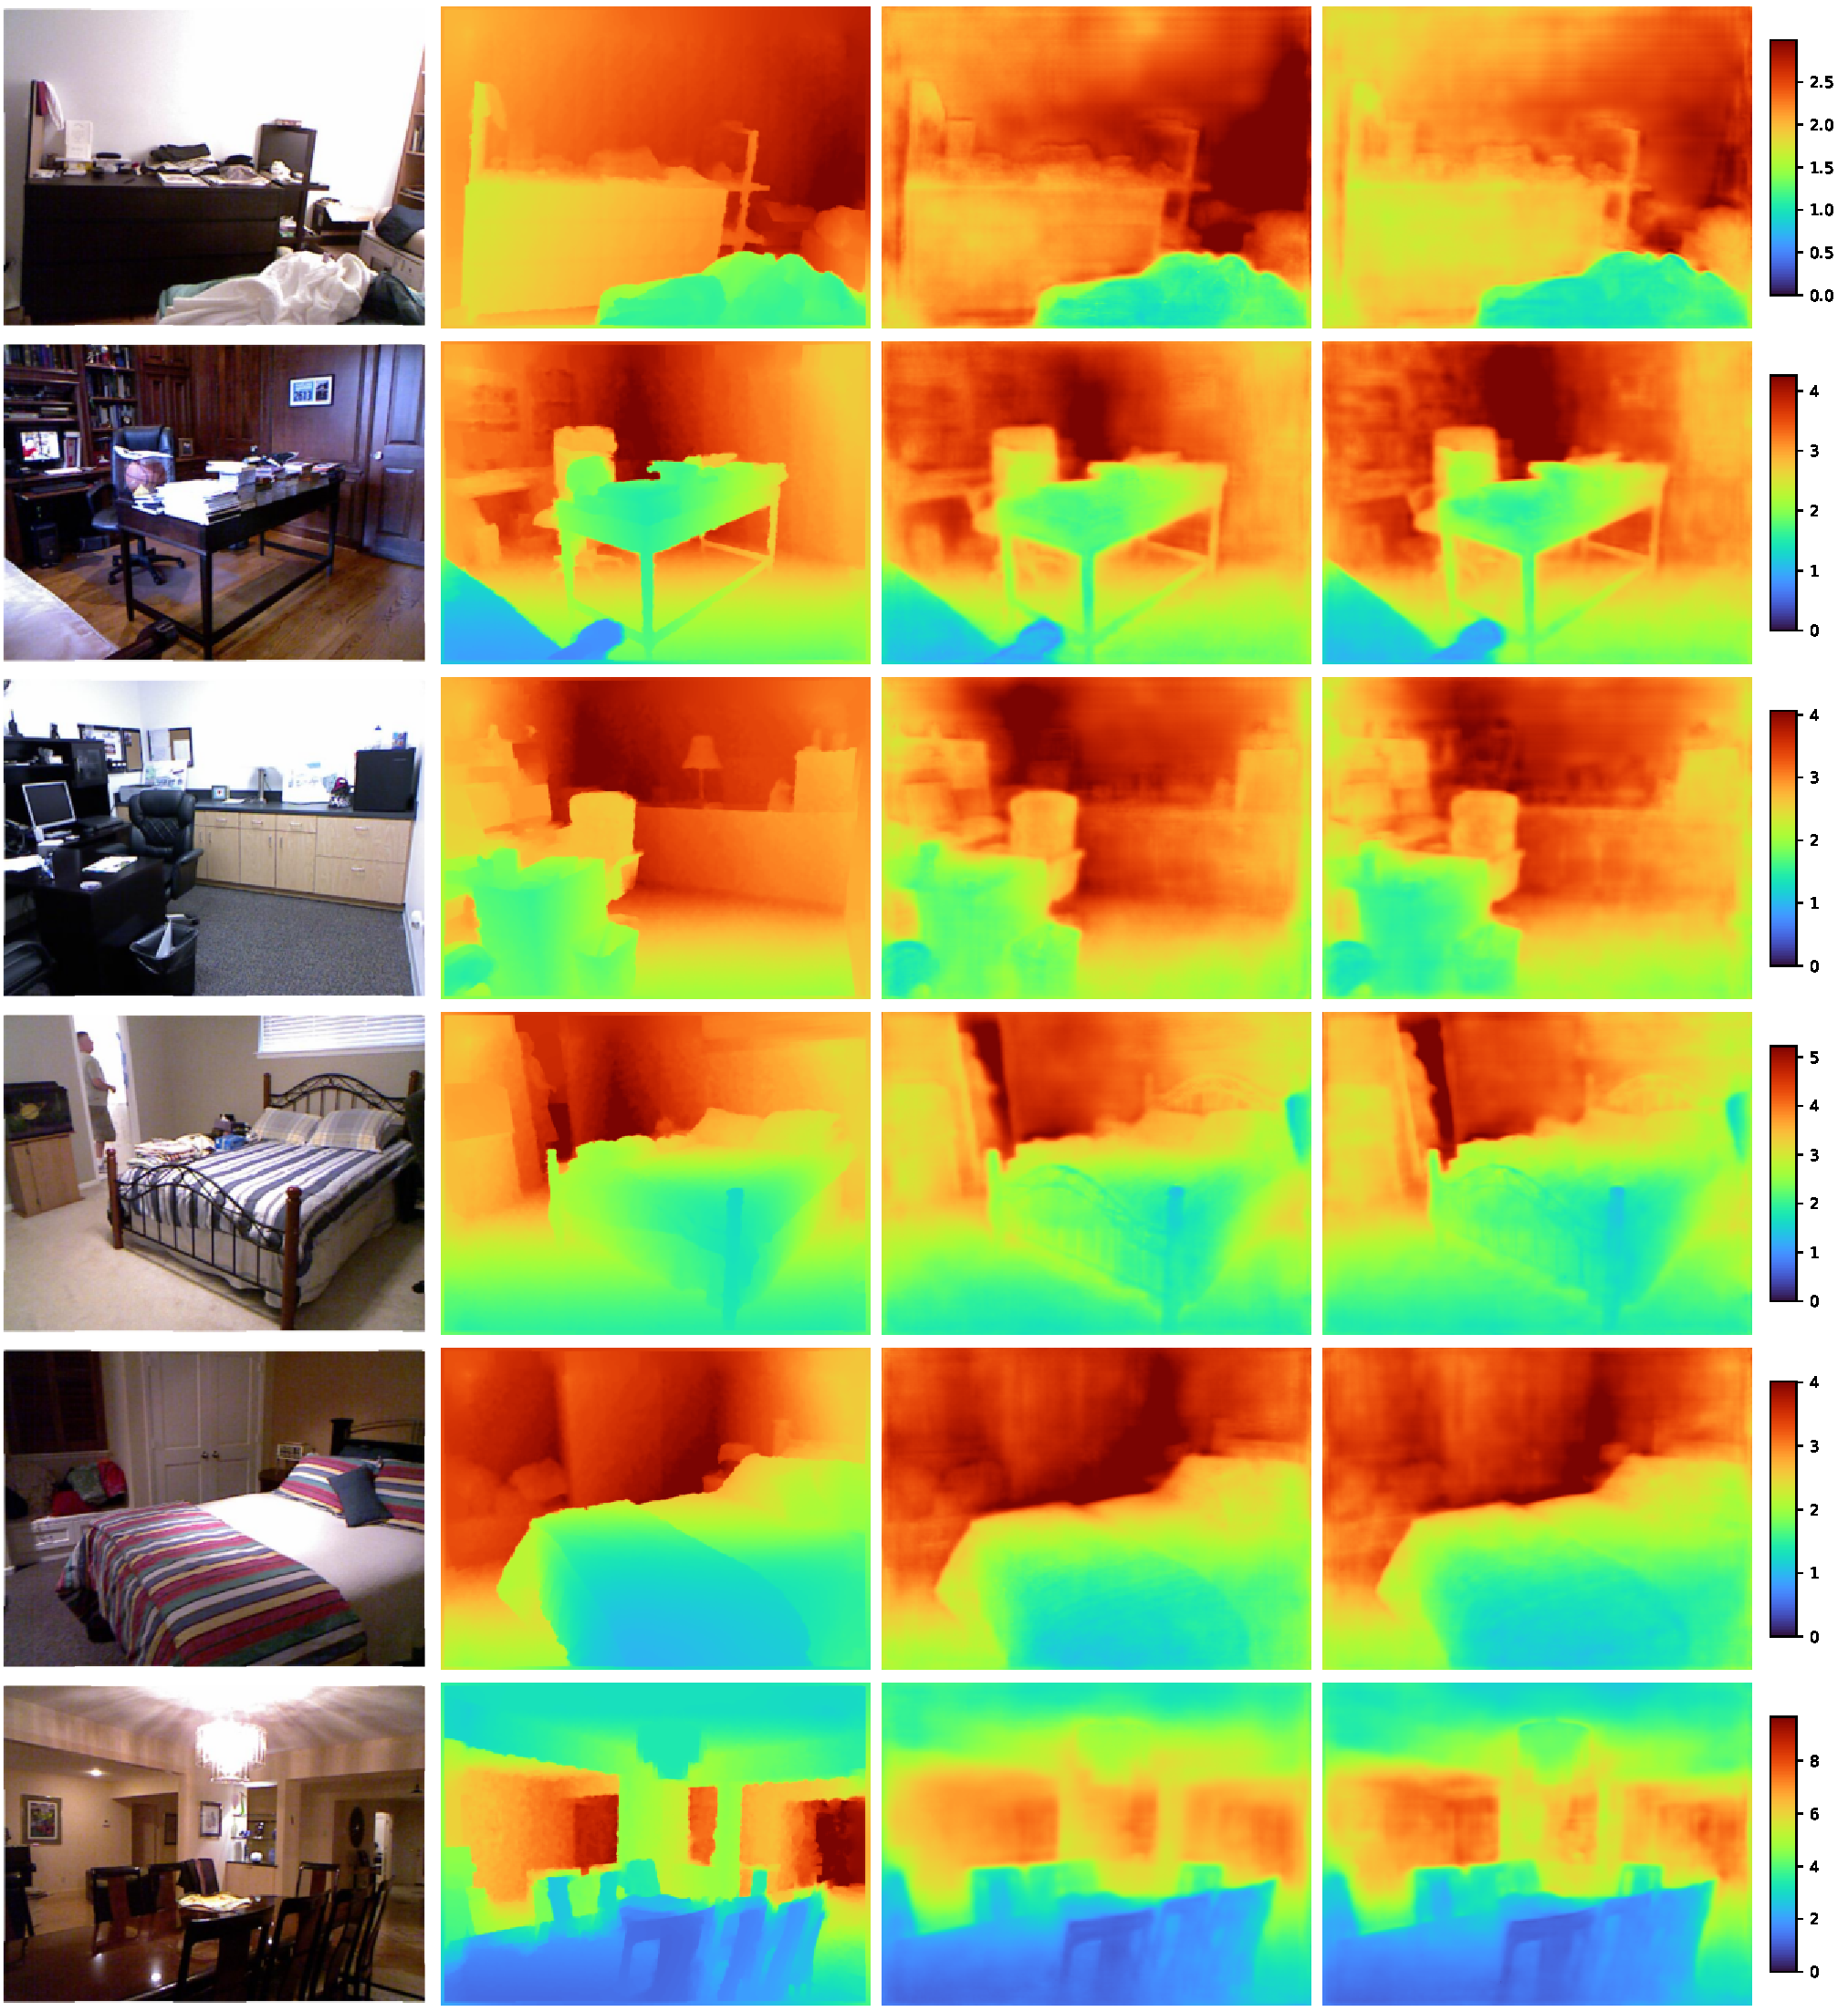
\includegraphics[width=\textwidth]{./figures/qualitative_depth_maps.pdf}};
        \node[thnote, anchor=south, font=\scriptsize\bfseries]
            at ([xshift=0.11625\textwidth]maps.north west) {تصویر ورودی};
        \node[thnote, anchor=south, font=\scriptsize\bfseries]
            at ([xshift=0.35475\textwidth]maps.north west) {عمق مرجع};
        \node[thnote, anchor=south, font=\scriptsize\bfseries, text=thControl]
            at ([xshift=0.59325\textwidth]maps.north west) {\tablecontrolmodel{} (فاقد \lr{K})};
        \node[thnote, anchor=south, font=\scriptsize\bfseries, text=thProposed]
            at ([xshift=0.83175\textwidth]maps.north west) {\tableproposedmodel{} (دارای \lr{K})};
    \end{tikzpicture}
    \caption[مقایسهٔ کیفی روی نمونهٔ پیش‌ثبت‌شده]{مقایسهٔ کیفی خروجی
    \proposedmodel{} و \controlmodel{} روی نمونه‌ای که \emph{پیش از هرگونه
    استنتاج} قفل شده است. شش تصویر تنها از روی بذر تصادفی \fadecimal{۲۰۲۶۰۸۲۱}
    از میان ۶۵۴ تصویر مجموعهٔ آزمون انتخاب شدند و چکیدهٔ \lr{SHA-256} فهرست
    شناسه‌ها (\lr{8086cb124e40}) پیش از بارگذاری هر مدل ثبت شد؛ بنابراین
    گزینش پس از مشاهدهٔ نتایج ممکن نبوده و شکل قابل ممیزی است. ستون‌ها از
    چپ به راست: تصویر ورودی، عمق مرجع، خروجی \controlmodel{} و خروجی
    \proposedmodel{}. در هر ردیف، نگاشت رنگ و بازهٔ عمق برای مرجع و هر دو
    مدل \emph{یکسان} است (نوار رنگ سمت راست همان ردیف، برحسب متر)، تا هیچ
    برتری بصری از نرمال‌سازی جداگانهٔ هر تصویر ناشی نشود. تفاوت دو مدل عمدتاً
    در \emph{مقیاس مطلق} صحنه است، نه در جزئیات ساختاری --- که با سازوکار
    پیش‌بینی‌شده در بخش~\ref{subsec:focal_jitter} هم‌خوان است.}
    \label{fig:qualitative_locked}
\end{figure}

\begin{figure}[htbp]
    \centering
    \begin{tikzpicture}
    \begin{axis}[
        thesisplot,
        width=0.86\textwidth, height=6.6cm,
        xlabel={نسبت مقیاس هر تصویر: میانهٔ پیش‌بینی تقسیم بر میانهٔ مرجع},
        ylabel={تعداد تصاویر},
        xmin=0.70, xmax=1.60, ymin=0, ymax=105,
        xtick={0.7,0.8,0.9,1.0,1.1,1.2,1.3,1.4,1.5,1.6},
        legend style={at={(0.97,0.97)}, anchor=north east},
        legend cell align=left,
    ]
    \addplot[ybar, bar width=0.0235, bar shift=0pt, draw=thProposed,
             fill=thProposed, fill opacity=0.55, draw opacity=0.9]
        table[x=center, y=proposed, col sep=space] {figures/curves/scale_ratio_hist.csv};
    \addlegendentry{\tableproposedmodel{}؛ میانه $1.015$}
    \addplot[ybar, bar width=0.0235, bar shift=0pt, draw=thControl,
             fill=thControl, fill opacity=0.45, draw opacity=0.9]
        table[x=center, y=control, col sep=space] {figures/curves/scale_ratio_hist.csv};
    \addlegendentry{\tablecontrolmodel{}؛ میانه $1.041$}
    % خط ایده‌آل با forget plot رسم می‌شود تا وارد فهرست راهنما نشود؛ برچسب آن
    % به‌صورت یک گره در کنار خط می‌آید.
    \addplot[draw=thIdeal, thick, dashed, forget plot]
        coordinates {(1.0,0) (1.0,105)};
    \node[thnote, anchor=west, text=thIdeal] at (axis cs:1.02,99) {ایده‌آل $1.000$};
    \end{axis}
    \end{tikzpicture}
    \caption[توزیع نسبت مقیاس هر تصویر]{توزیع نسبت مقیاس هر تصویر روی
    \emph{تمام} ۶۵۴ تصویر مجموعهٔ آزمون --- همان نمونه‌ای که آزمون‌های زوجی
    بخش~\ref{subsec:focal_jitter} روی آن انجام شده است. مقدار ایده‌آل ۱ است.
    این نمودار سازوکار عددی برتری گزارش‌شده در
    جدول~\ref{tab:nyu_metric_focal} را آشکار می‌کند: توزیع \proposedmodel{}
    هم نزدیک‌تر به مقدار ایده‌آل است (میانه \fadecimal{۱٫۰۱۵} در برابر
    \fadecimal{۱٫۰۴۱}) و هم فشرده‌تر (انحراف معیار \fadecimal{۰٫۰۷۸} در برابر
    \fadecimal{۰٫۰۹۴}؛ دامنهٔ میان‌چارکی \fadecimal{۰٫۰۹۸} در برابر
    \fadecimal{۰٫۱۱۴}). به بیان دیگر، \controlmodel{} --- که ناچار است به
    میانگین توزیع $\alpha$ رگرسیون کند --- هم اریب است و هم پراکنده‌تر، دقیقاً
    همان‌گونه که تحلیل بدساختی مسئله پیش‌بینی می‌کرد. در سطح تک‌تصویر نیز،
    \proposedmodel{} در ۳۹۹ تصویر از ۶۵۴ تصویر (۶۱ درصد) به مقیاس صحیح
    نزدیک‌تر است.}
    \label{fig:scale_ratio_distribution}
\end{figure}

%
% سرستون‌های فارسی در همین‌جا حروف‌چینی می‌شوند (نه داخل تصویر)، تا با
% تایپوگرافی بقیهٔ پایان‌نامه یکسان باشند. کسرهای افقی زیر، دقیقاً همان
% COLUMN_CENTRES در tools/make_qualitative_figure.py هستند؛ اگر هندسهٔ آن
% اسکریپت تغییر کند، این چهار عدد نیز باید به‌روزرسانی شوند.
% =============================================================================

\begin{figure}[htbp]
    \centering
    \begin{tikzpicture}
        \node[anchor=south west, inner sep=0pt] (maps)
            {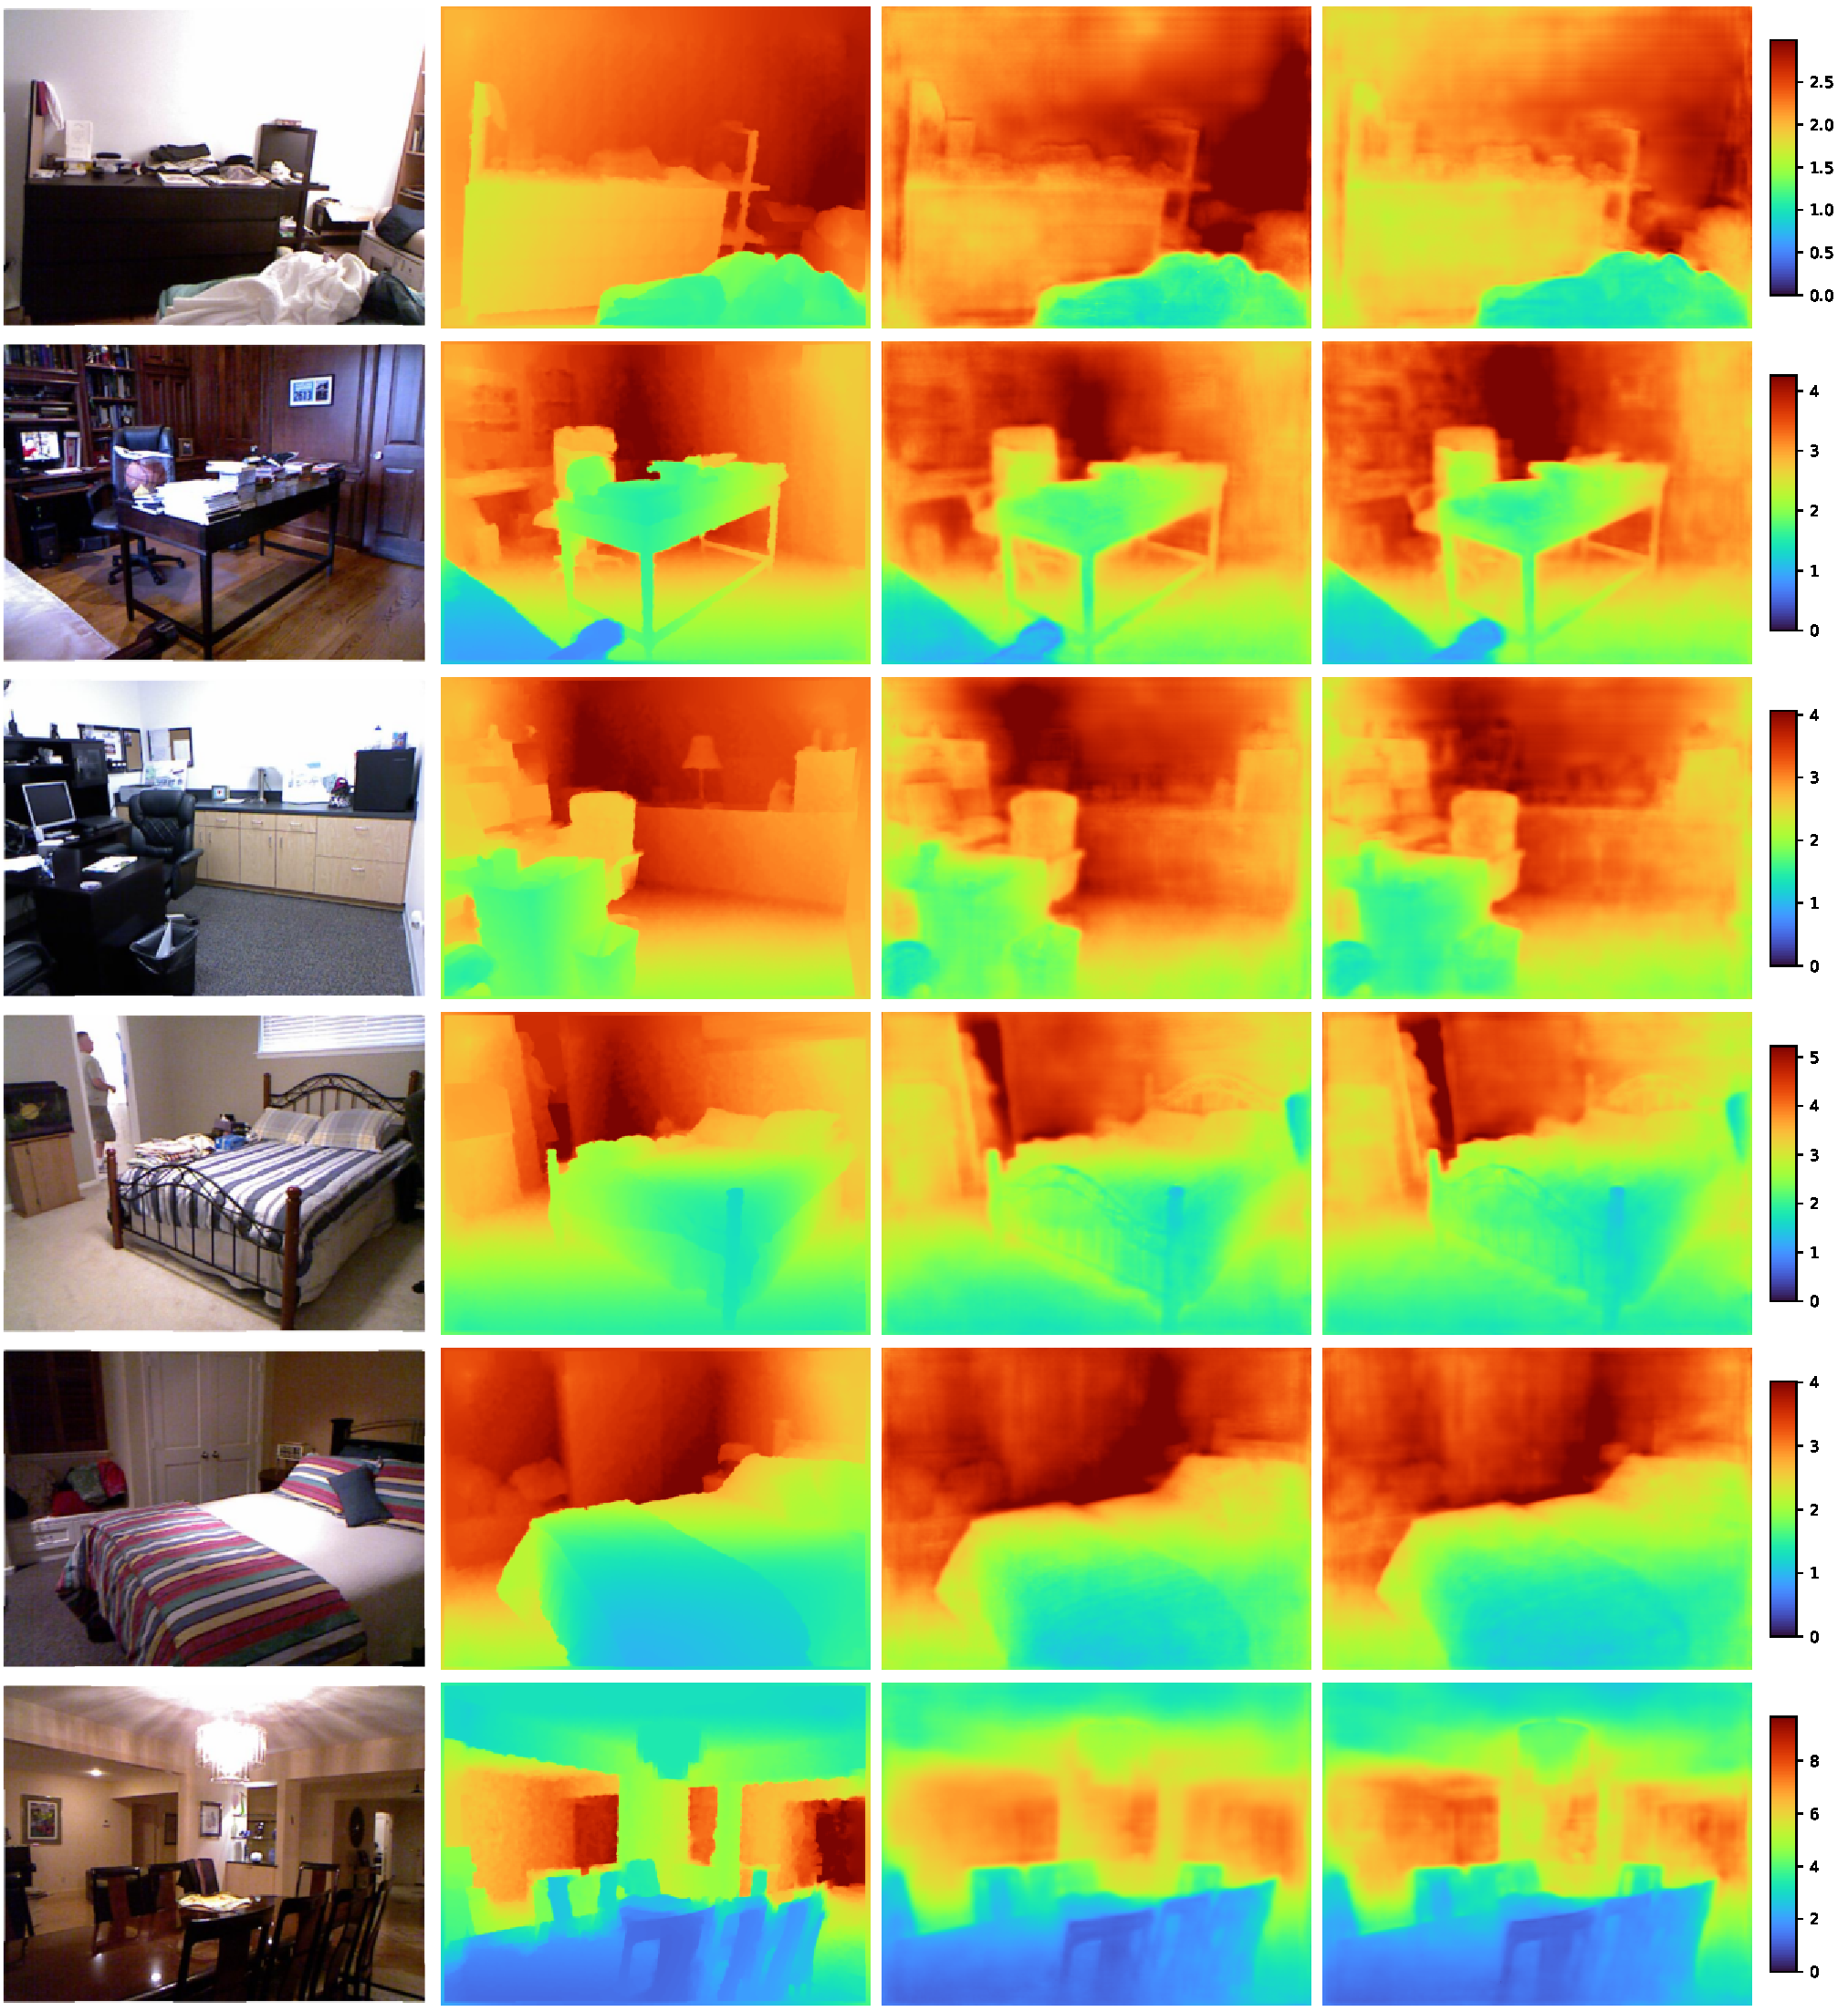
\includegraphics[width=\textwidth]{./figures/qualitative_depth_maps.pdf}};
        \node[thnote, anchor=south, font=\scriptsize\bfseries]
            at ([xshift=0.11625\textwidth]maps.north west) {تصویر ورودی};
        \node[thnote, anchor=south, font=\scriptsize\bfseries]
            at ([xshift=0.35475\textwidth]maps.north west) {عمق مرجع};
        \node[thnote, anchor=south, font=\scriptsize\bfseries, text=thControl]
            at ([xshift=0.59325\textwidth]maps.north west) {\tablecontrolmodel{} (فاقد \lr{K})};
        \node[thnote, anchor=south, font=\scriptsize\bfseries, text=thProposed]
            at ([xshift=0.83175\textwidth]maps.north west) {\tableproposedmodel{} (دارای \lr{K})};
    \end{tikzpicture}
    \caption[مقایسهٔ کیفی روی نمونهٔ پیش‌ثبت‌شده]{مقایسهٔ کیفی خروجی
    \proposedmodel{} و \controlmodel{} روی نمونه‌ای که \emph{پیش از هرگونه
    استنتاج} قفل شده است. شش تصویر تنها از روی بذر تصادفی \fadecimal{۲۰۲۶۰۸۲۱}
    از میان ۶۵۴ تصویر مجموعهٔ آزمون انتخاب شدند و چکیدهٔ \lr{SHA-256} فهرست
    شناسه‌ها (\lr{8086cb124e40}) پیش از بارگذاری هر مدل ثبت شد؛ بنابراین
    گزینش پس از مشاهدهٔ نتایج ممکن نبوده و شکل قابل ممیزی است. ستون‌ها از
    چپ به راست: تصویر ورودی، عمق مرجع، خروجی \controlmodel{} و خروجی
    \proposedmodel{}. در هر ردیف، نگاشت رنگ و بازهٔ عمق برای مرجع و هر دو
    مدل \emph{یکسان} است (نوار رنگ سمت راست همان ردیف، برحسب متر)، تا هیچ
    برتری بصری از نرمال‌سازی جداگانهٔ هر تصویر ناشی نشود. تفاوت دو مدل عمدتاً
    در \emph{مقیاس مطلق} صحنه است، نه در جزئیات ساختاری --- که با سازوکار
    پیش‌بینی‌شده در بخش~\ref{subsec:focal_jitter} هم‌خوان است.}
    \label{fig:qualitative_locked}
\end{figure}

\begin{figure}[htbp]
    \centering
    \begin{tikzpicture}
    \begin{axis}[
        thesisplot,
        width=0.86\textwidth, height=6.6cm,
        xlabel={نسبت مقیاس هر تصویر: میانهٔ پیش‌بینی تقسیم بر میانهٔ مرجع},
        ylabel={تعداد تصاویر},
        xmin=0.70, xmax=1.60, ymin=0, ymax=105,
        xtick={0.7,0.8,0.9,1.0,1.1,1.2,1.3,1.4,1.5,1.6},
        legend style={at={(0.97,0.97)}, anchor=north east},
        legend cell align=left,
    ]
    \addplot[ybar, bar width=0.0235, bar shift=0pt, draw=thProposed,
             fill=thProposed, fill opacity=0.55, draw opacity=0.9]
        table[x=center, y=proposed, col sep=space] {figures/curves/scale_ratio_hist.csv};
    \addlegendentry{\tableproposedmodel{}؛ میانه $1.015$}
    \addplot[ybar, bar width=0.0235, bar shift=0pt, draw=thControl,
             fill=thControl, fill opacity=0.45, draw opacity=0.9]
        table[x=center, y=control, col sep=space] {figures/curves/scale_ratio_hist.csv};
    \addlegendentry{\tablecontrolmodel{}؛ میانه $1.041$}
    % خط ایده‌آل با forget plot رسم می‌شود تا وارد فهرست راهنما نشود؛ برچسب آن
    % به‌صورت یک گره در کنار خط می‌آید.
    \addplot[draw=thIdeal, thick, dashed, forget plot]
        coordinates {(1.0,0) (1.0,105)};
    \node[thnote, anchor=west, text=thIdeal] at (axis cs:1.02,99) {ایده‌آل $1.000$};
    \end{axis}
    \end{tikzpicture}
    \caption[توزیع نسبت مقیاس هر تصویر]{توزیع نسبت مقیاس هر تصویر روی
    \emph{تمام} ۶۵۴ تصویر مجموعهٔ آزمون --- همان نمونه‌ای که آزمون‌های زوجی
    بخش~\ref{subsec:focal_jitter} روی آن انجام شده است. مقدار ایده‌آل ۱ است.
    این نمودار سازوکار عددی برتری گزارش‌شده در
    جدول~\ref{tab:nyu_metric_focal} را آشکار می‌کند: توزیع \proposedmodel{}
    هم نزدیک‌تر به مقدار ایده‌آل است (میانه \fadecimal{۱٫۰۱۵} در برابر
    \fadecimal{۱٫۰۴۱}) و هم فشرده‌تر (انحراف معیار \fadecimal{۰٫۰۷۸} در برابر
    \fadecimal{۰٫۰۹۴}؛ دامنهٔ میان‌چارکی \fadecimal{۰٫۰۹۸} در برابر
    \fadecimal{۰٫۱۱۴}). به بیان دیگر، \controlmodel{} --- که ناچار است به
    میانگین توزیع $\alpha$ رگرسیون کند --- هم اریب است و هم پراکنده‌تر، دقیقاً
    همان‌گونه که تحلیل بدساختی مسئله پیش‌بینی می‌کرد. در سطح تک‌تصویر نیز،
    \proposedmodel{} در ۳۹۹ تصویر از ۶۵۴ تصویر (۶۱ درصد) به مقیاس صحیح
    نزدیک‌تر است.}
    \label{fig:scale_ratio_distribution}
\end{figure}
